\documentclass{article}
\usepackage{indentfirst}
\setlength{\parindent}{2em}
\usepackage{graphicx}

\title{SYSC 5001W: Project deliverable 2} % Title of the assignment

\author{Qiguang Chu\\ \texttt{300042722}} % Author name and email address

\date{University of Ottawa --- \today} % University, school and/or department name(s) and a date

%----------------------------------------------------------------------------------------

\begin{document}

\maketitle

\section{Model Verification and Validation}

The goal of the validation is to produce a model that represents true system behavior closely enough for the model
to be used as a substitute for the actual system. 

\subsection{Verification of Simulation Models}

Verification is concerned with building the model correctly. It proceeds by the comparison of the conceptual model to the computer representation what implements that conception.

\subsubsection{Flow Diagram}
I made a flow diagram that includes each logically possible action a system can take when an event occurs.

\begin{figure}[htbp]
\begin{center}
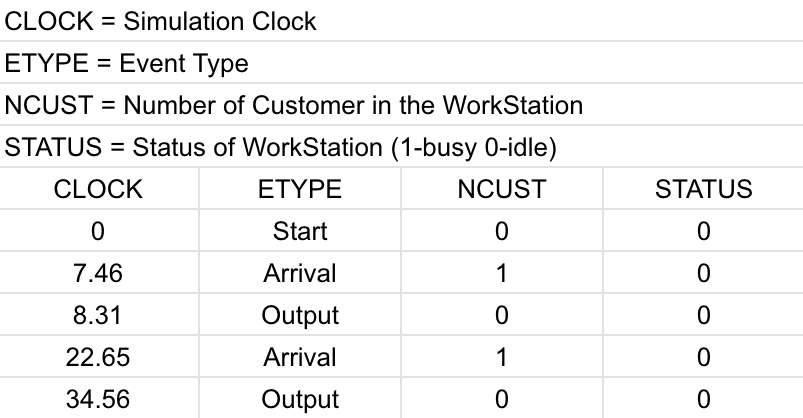
\includegraphics[width=4in]{Simulationtrace.png}
\caption{Simulation Trace}
\label{default}
\end{center}
\end{figure}

\begin{figure}[htbp]
\begin{center}
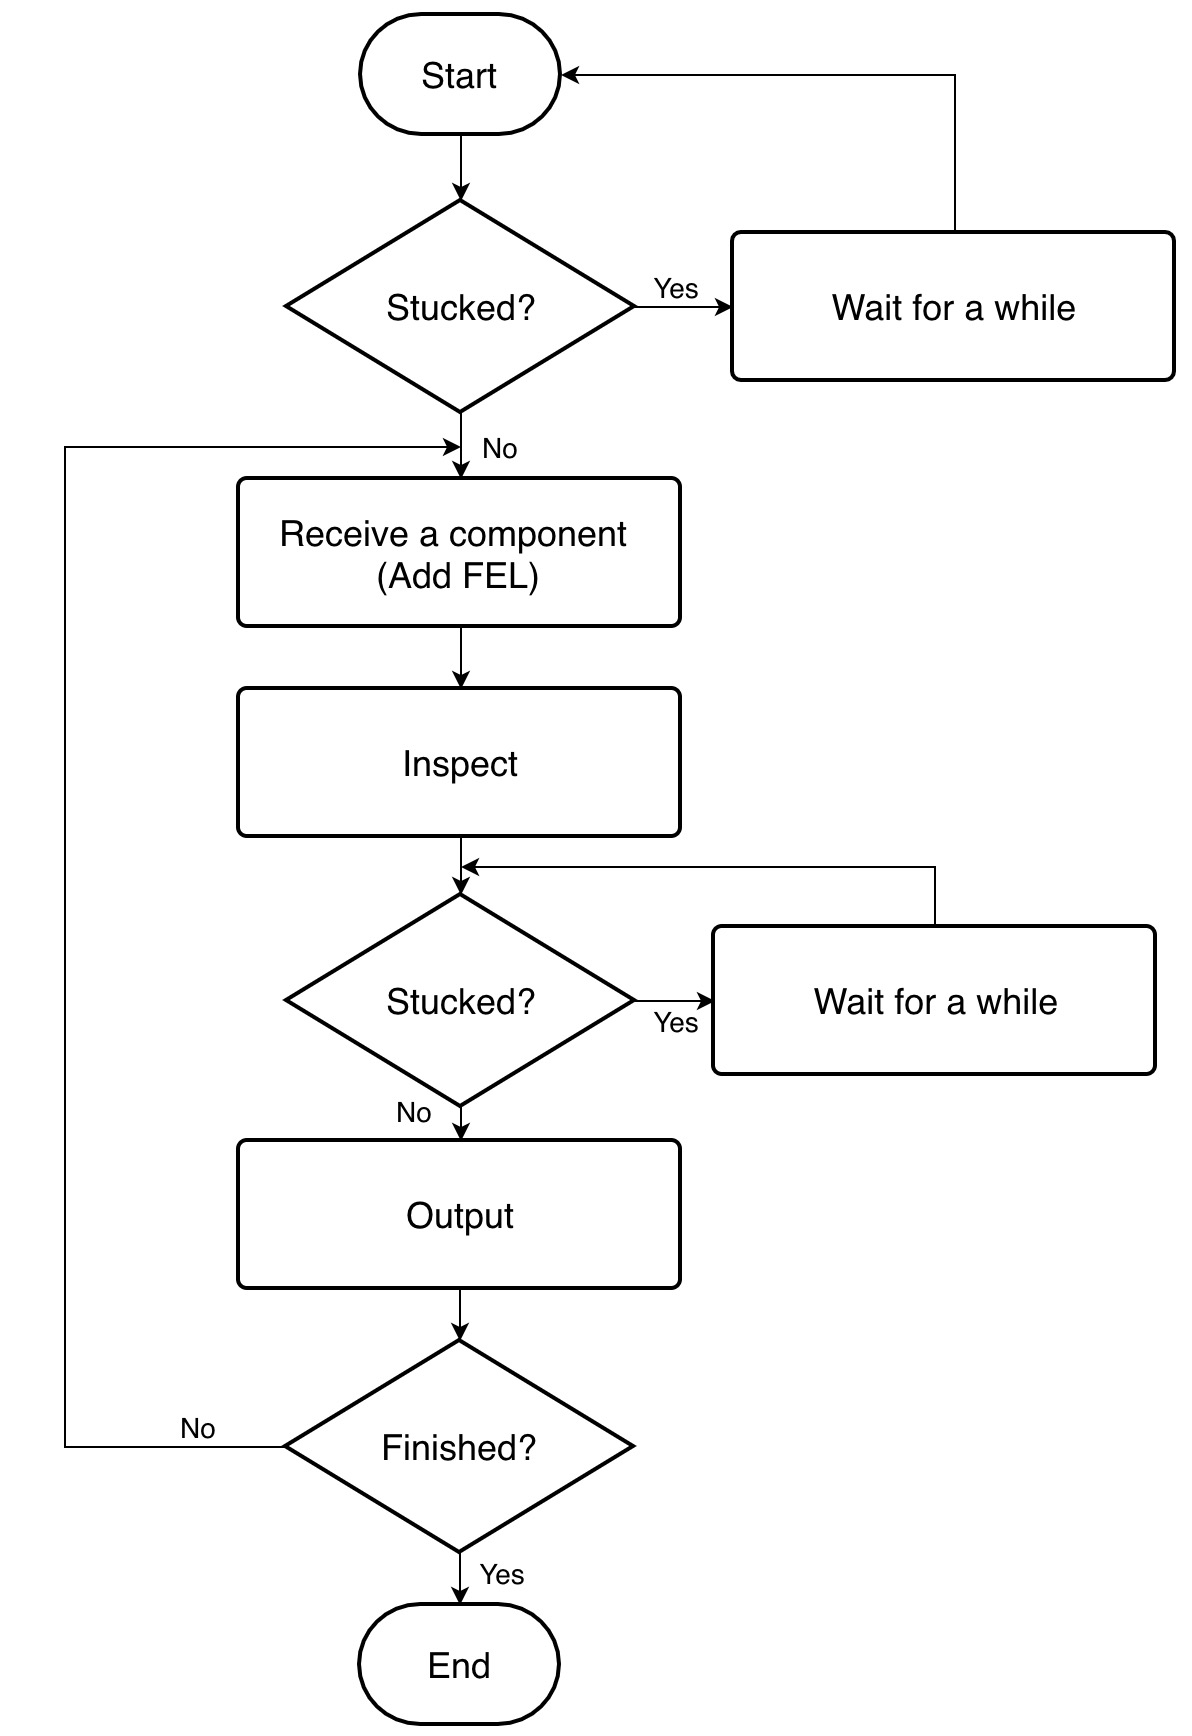
\includegraphics[width=4in]{Flowchartsp.png}
\caption{Work flow of Inspectors}
\label{default}
\end{center}
\end{figure}

\begin{figure}[htbp]
\begin{center}
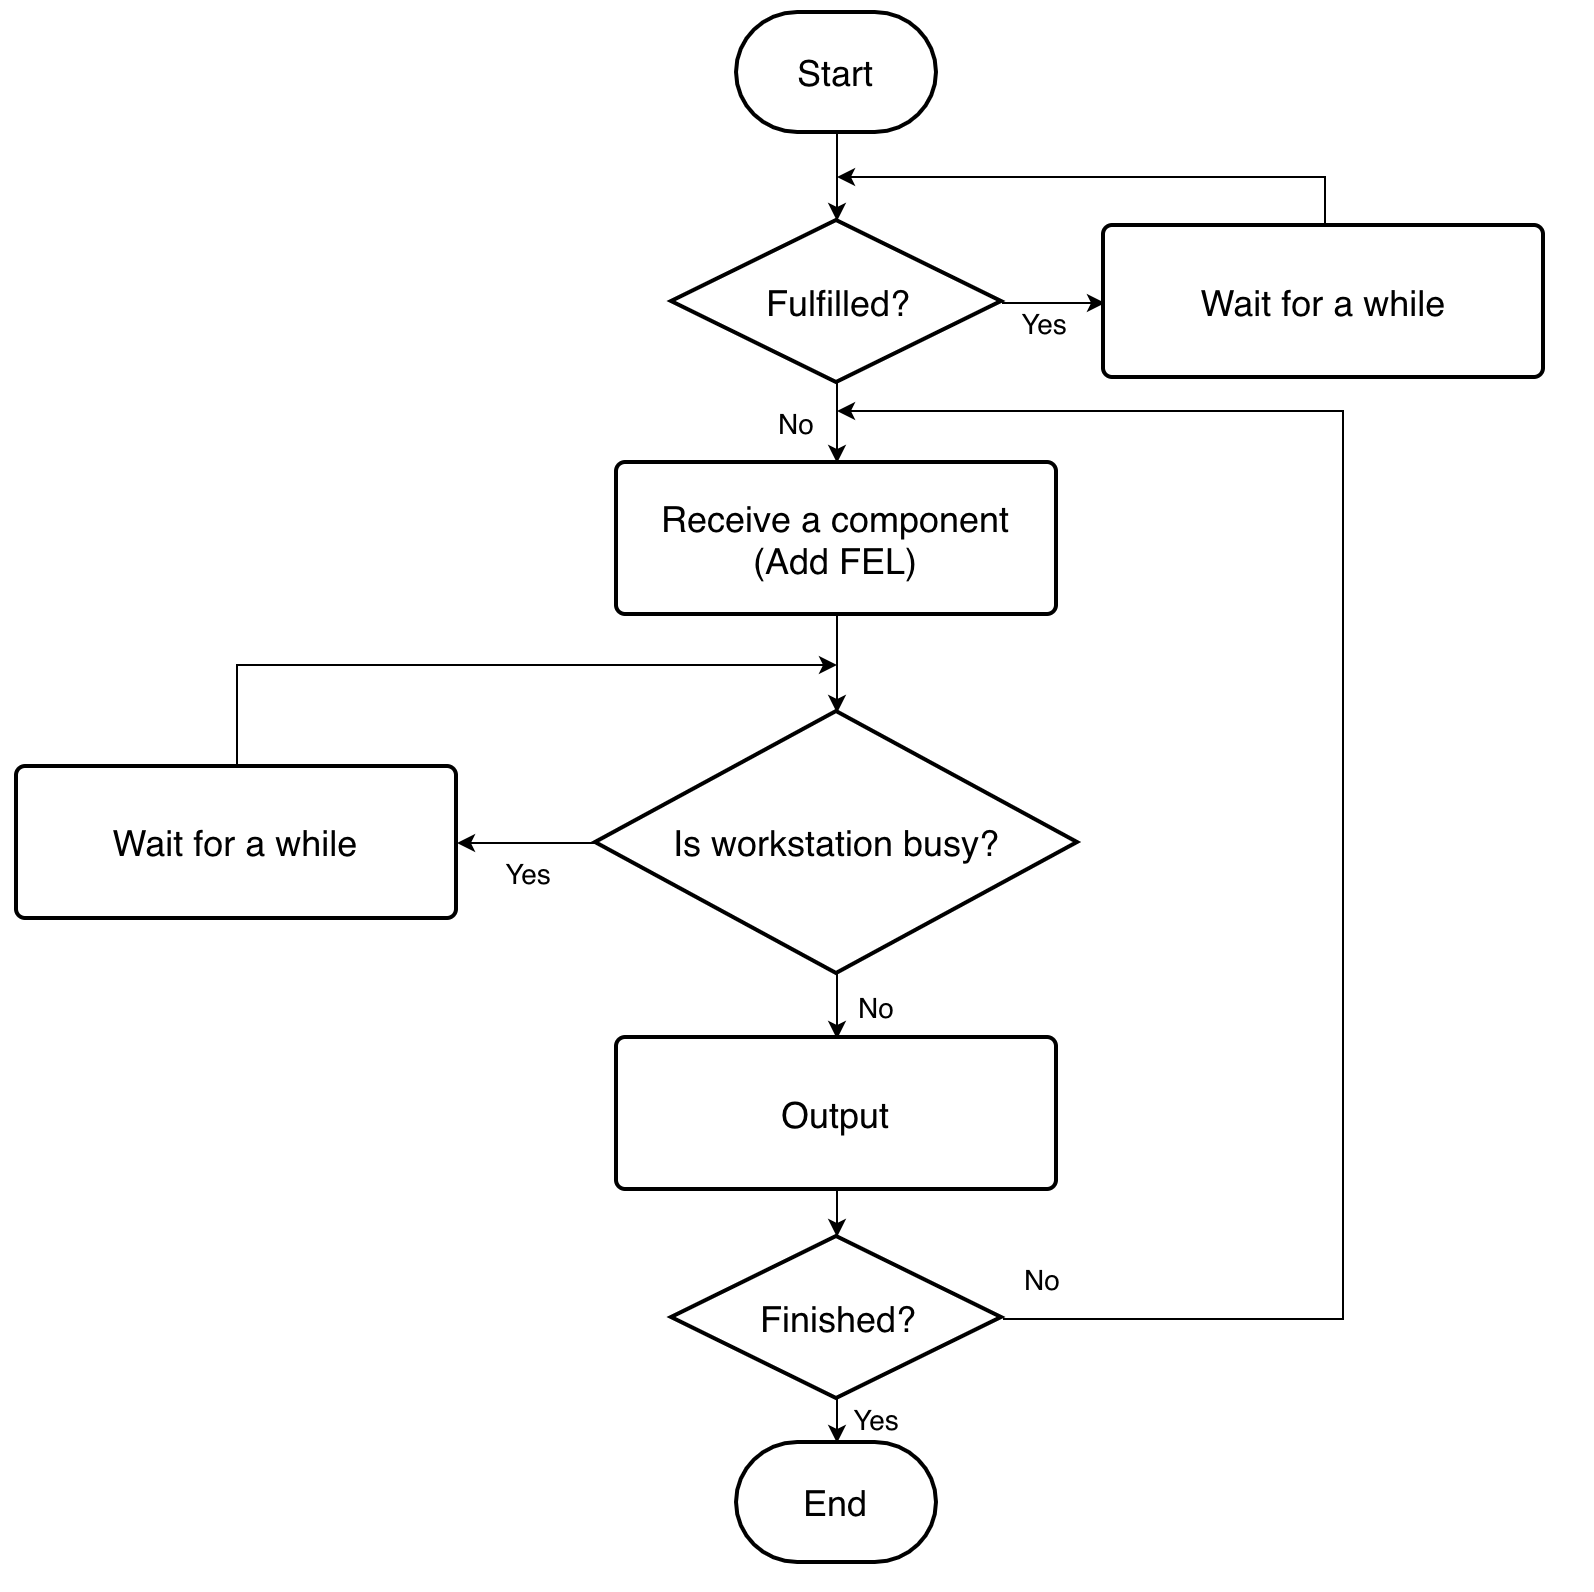
\includegraphics[width=4in]{Flowchartbuffer.png}
\caption{Work flow of Buffer}
\label{default}
\end{center}
\end{figure}

\begin{figure}[htbp]
\begin{center}
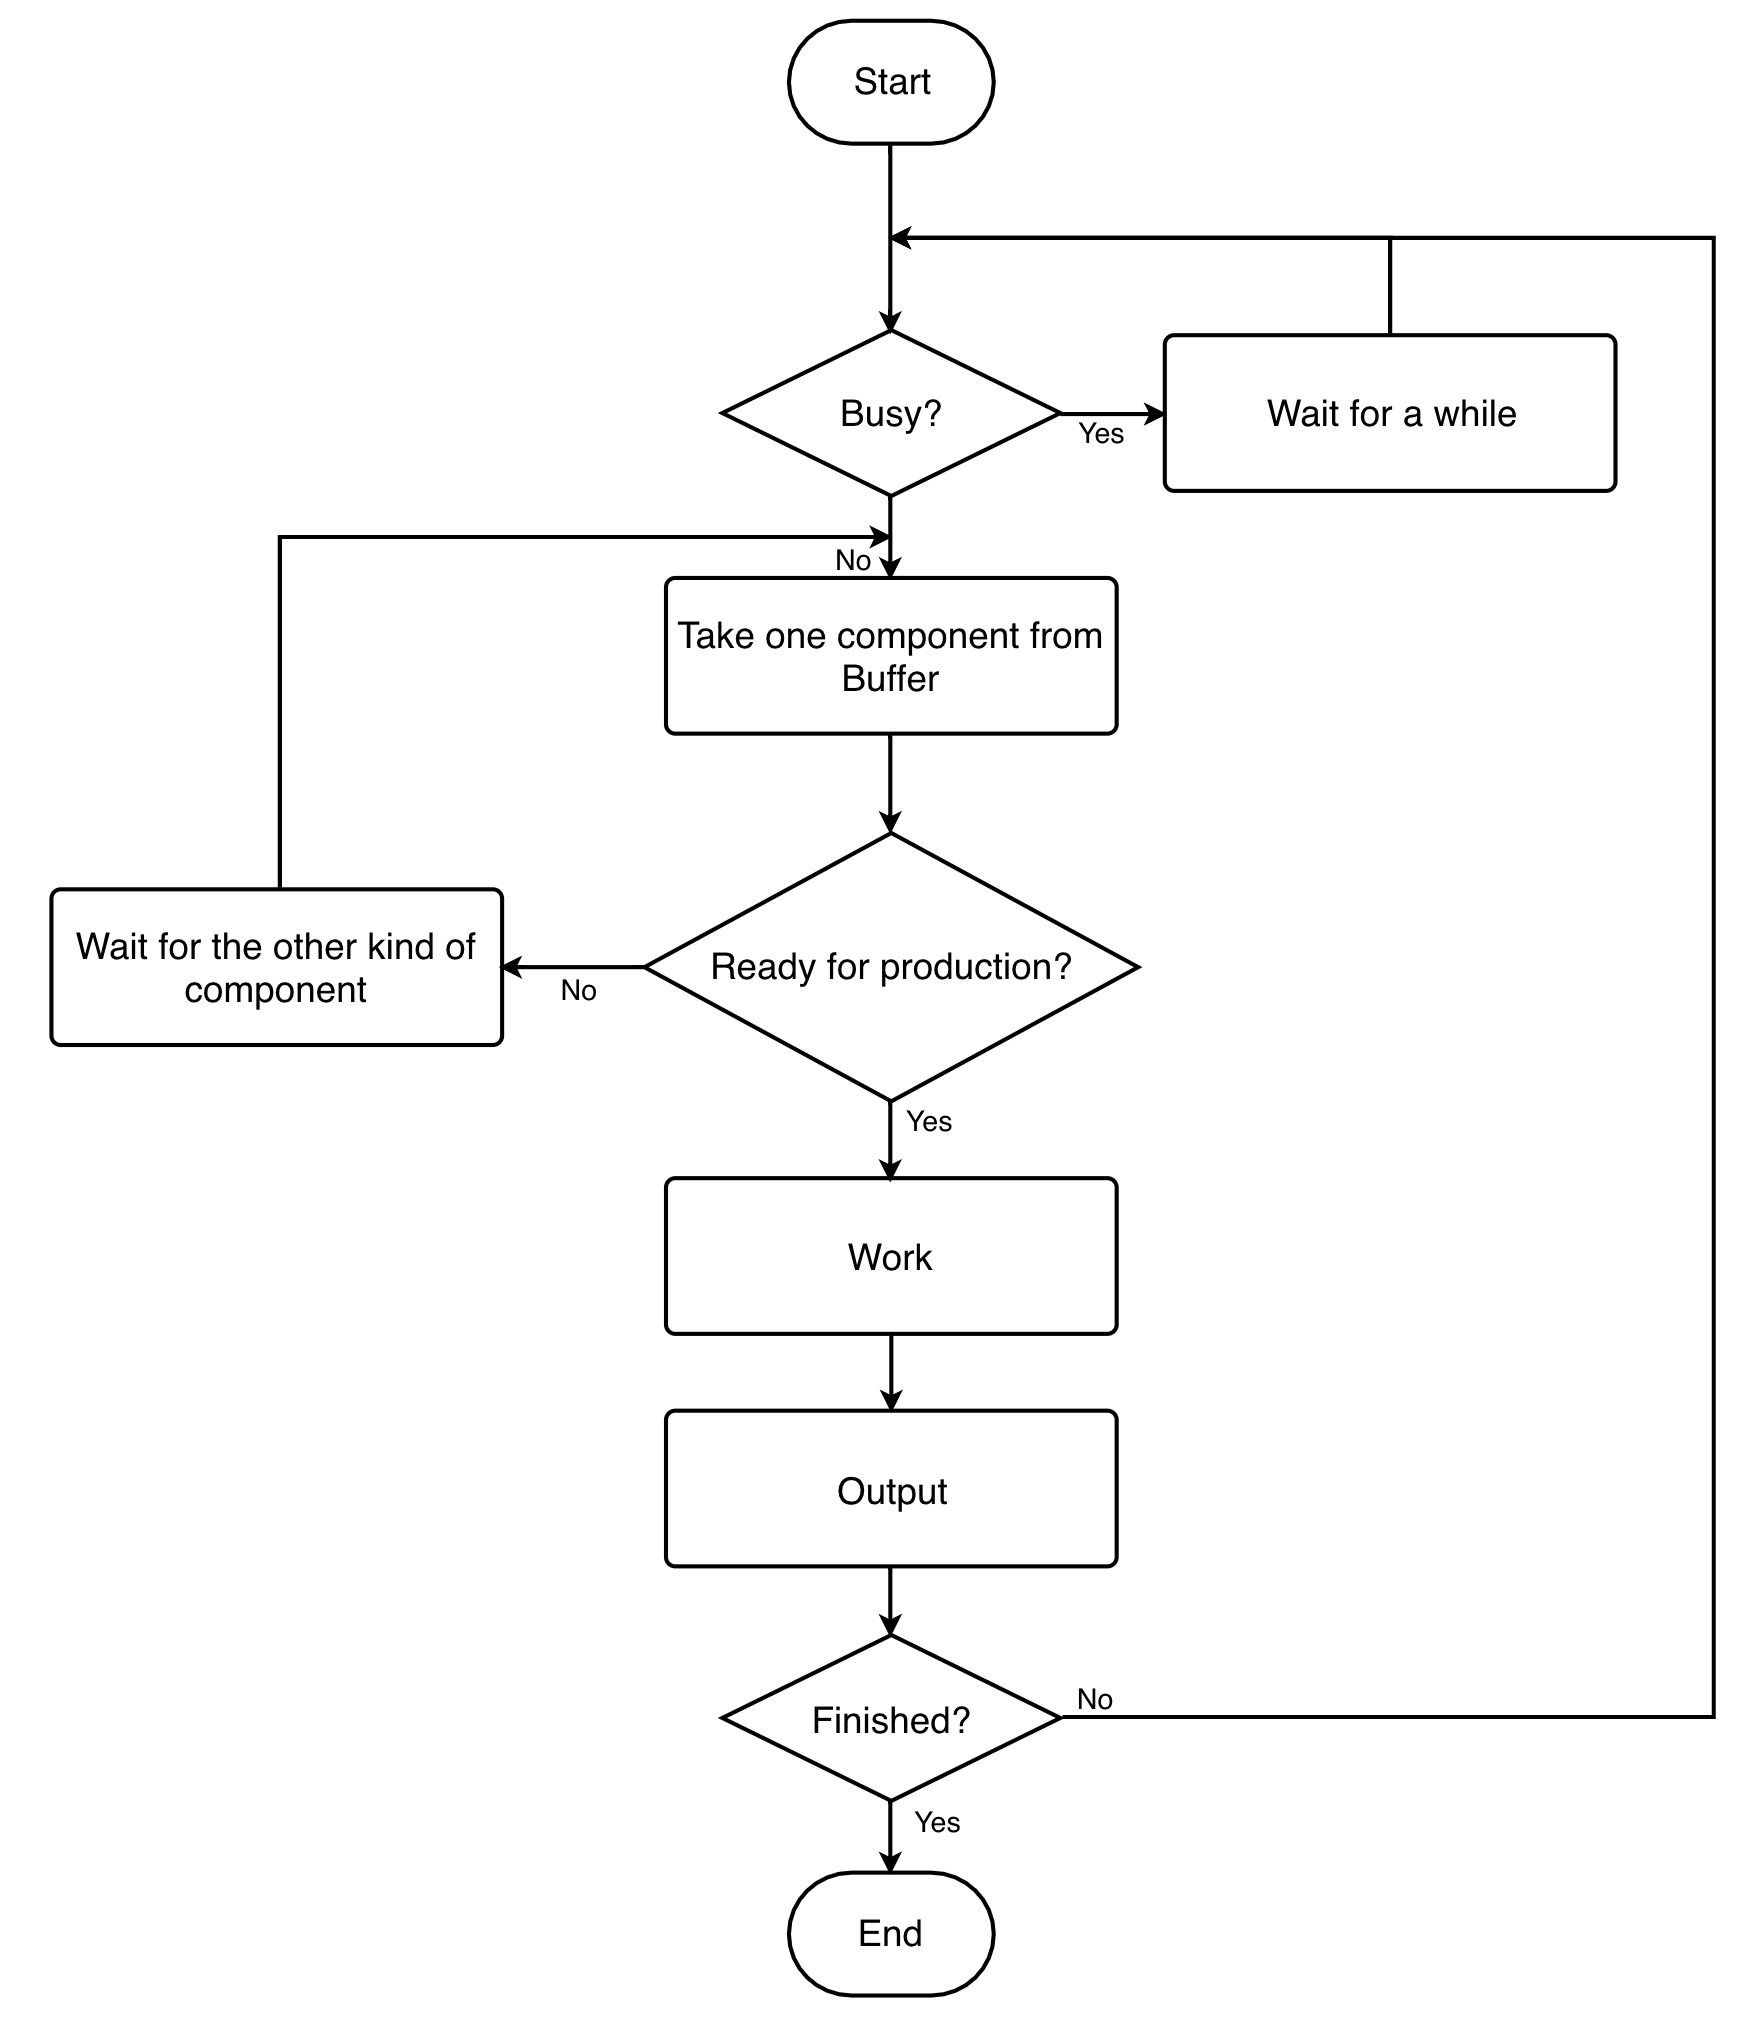
\includegraphics[width=4in]{Flowchartws.png}
\caption{Work flow of Workstation}
\label{default}
\end{center}
\end{figure}


This simulation trace table indicates how the Workstation 1 work in this process. It just wait for Component 1, deal with it and then output. If the station is busy and a new one comes, the new arrival will stay at the buffer for now.

\subsubsection{Model Output}

The output of model is reasonable because it tracks each component of the whole process and the total time it costs is similar to the real time cost. For each object in the process, I can extract what it is doing at a certain point in time.

\subsubsection{Sequence of dealing events}

My code follows the rule that proceed events as time goes. The primary key of every event happened in this process is the clock. When we know that something is certain to happen, we put it in the FEL. Then we sort it according to the time of the occurrence of these things. The earlier event comes out first and latter event comes out the last. 

\subsubsection{Little's Law}

Little's Law works for any blackbox, where the blackbox can be a complex system, or  any subunit such as a single waiting line or a single server, a waiting line plus a sever, etc. 

For each queue system in this project, we do a Little's law verification.
\begin{equation}
\hat L = \hat \lambda \hat w
\end{equation}
$\hat L$ means average number of components in the queue. $\hat \lambda$ means the arrival rate of components. $\hat w$ means average working time for each component.

For Inspector system, consider the supply of the component for each inspector is sufficient, which means theres always a component waiting outside and there's always existing one component in each inspector. It's easy to calculate that the average dealing time for each inspector but things are little different here. If the corresponding workstation has a full buffer already and can't hold more components, the component must stay in the inspector and the inspector stop receiving new components. Here we have $L=\hat L =1, \hat w = 10.36, \hat \lambda = 0.10$. It follows Little's law. By checking to see if these averages are in range, we can verify quickly if the system is wrong before we even look at any other part of the simulation.
Here we have the number of each component in each buffer of the specific workstation.

\begin{figure}[htbp]
\begin{center}
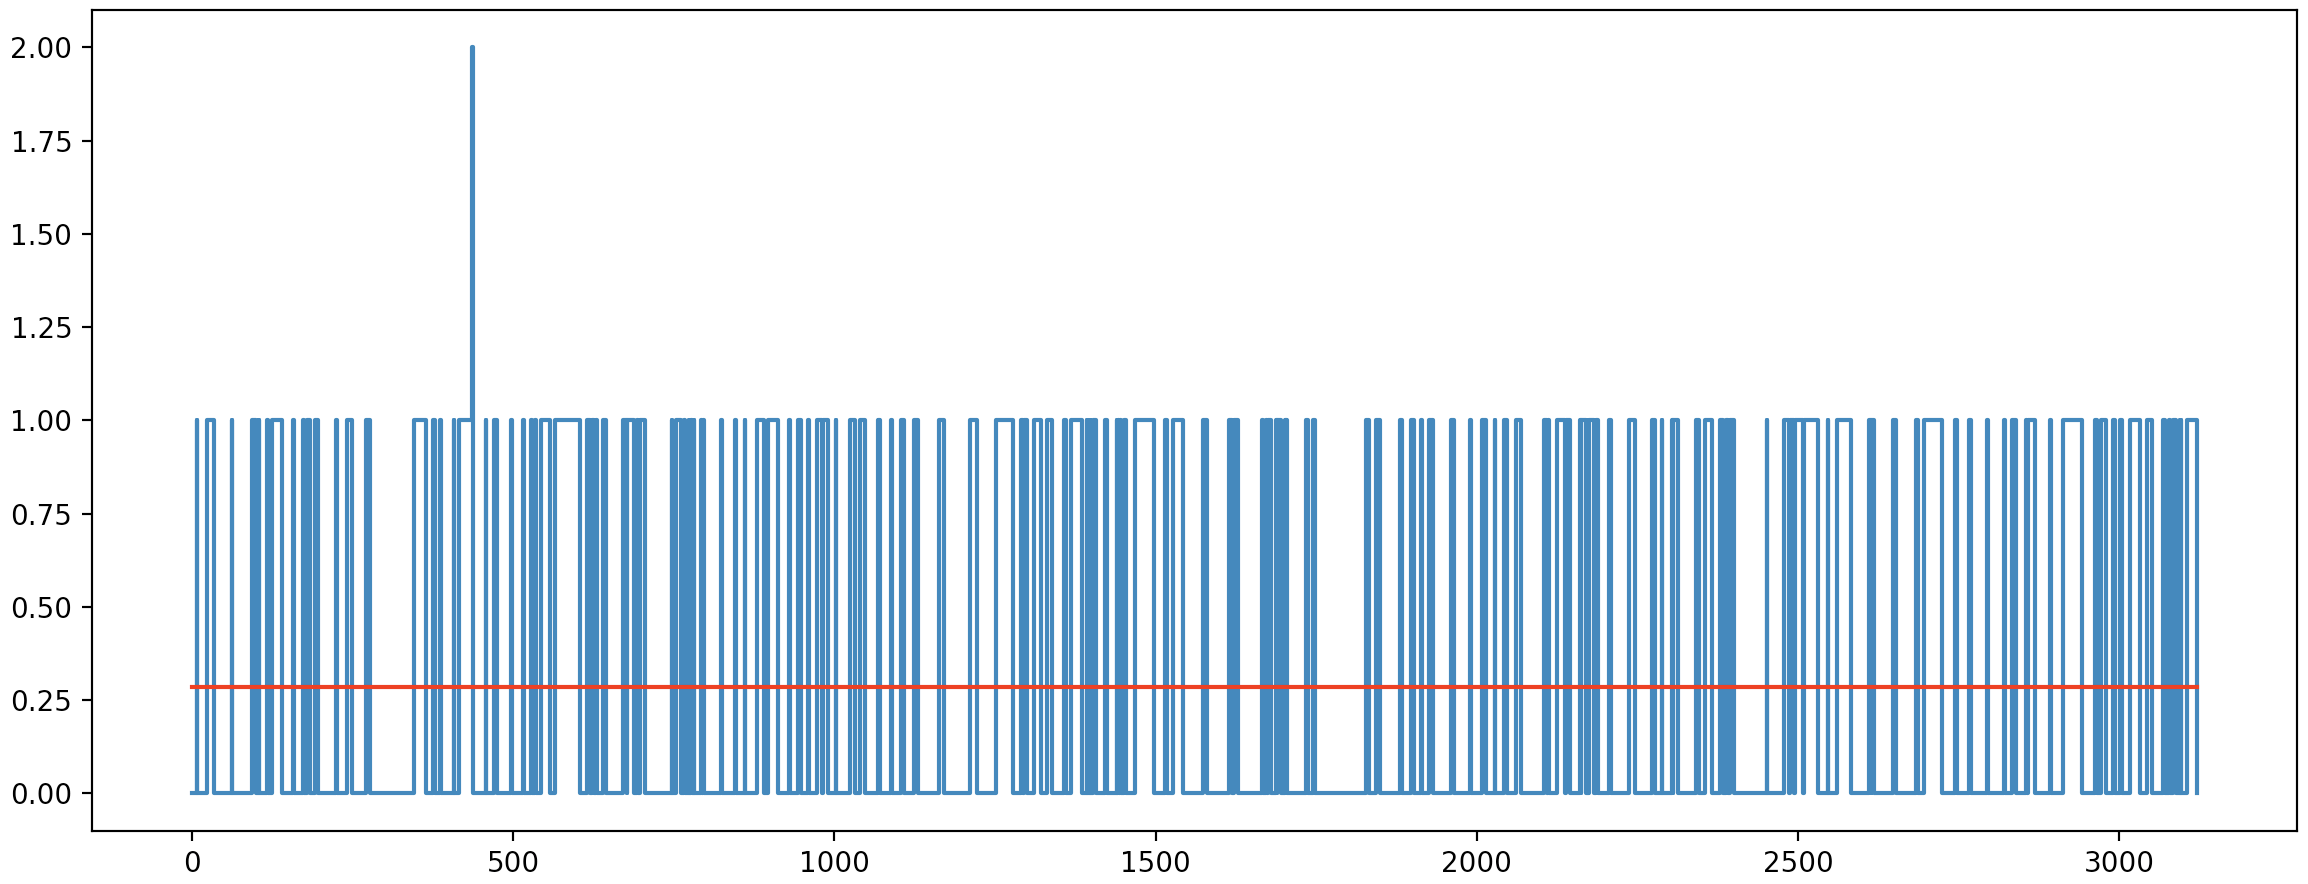
\includegraphics[width=4in]{W1_C1B.png}
\caption{The number of components in Component 1 buffer of Workstation 1}
\label{W1_C1B}
\end{center}
\end{figure}

The x axle on the diagram shows the time line of the whole process of production, while the y axle indicates how many kind of this components in the buffer at this time. I also draw a red line to denote the average number of gears in buffer in this period. It has to be mentioned that I ignored the case that the workstation receive the component and then immediately use it to produce. That is because the time component stay in buffer is extremely slow and we can see it as no change in the buffer. By the way, in order to get rid of error, we must promise all buffers of workstations are empty when the simulation ends, which is as same as the beginning. The time point in this simulation is T = 2713.501

Component 1 buffer of Workstation 1:

Verification: $L = 0.109, \lambda = 0.037, w = 2.979, T = 2713.501$
\begin{equation}
\lambda w = 0.037*2.979 = 0.109 = L
\end{equation}

This queue pass the Little's law verification.

\begin{figure}[htbp]
\begin{center}
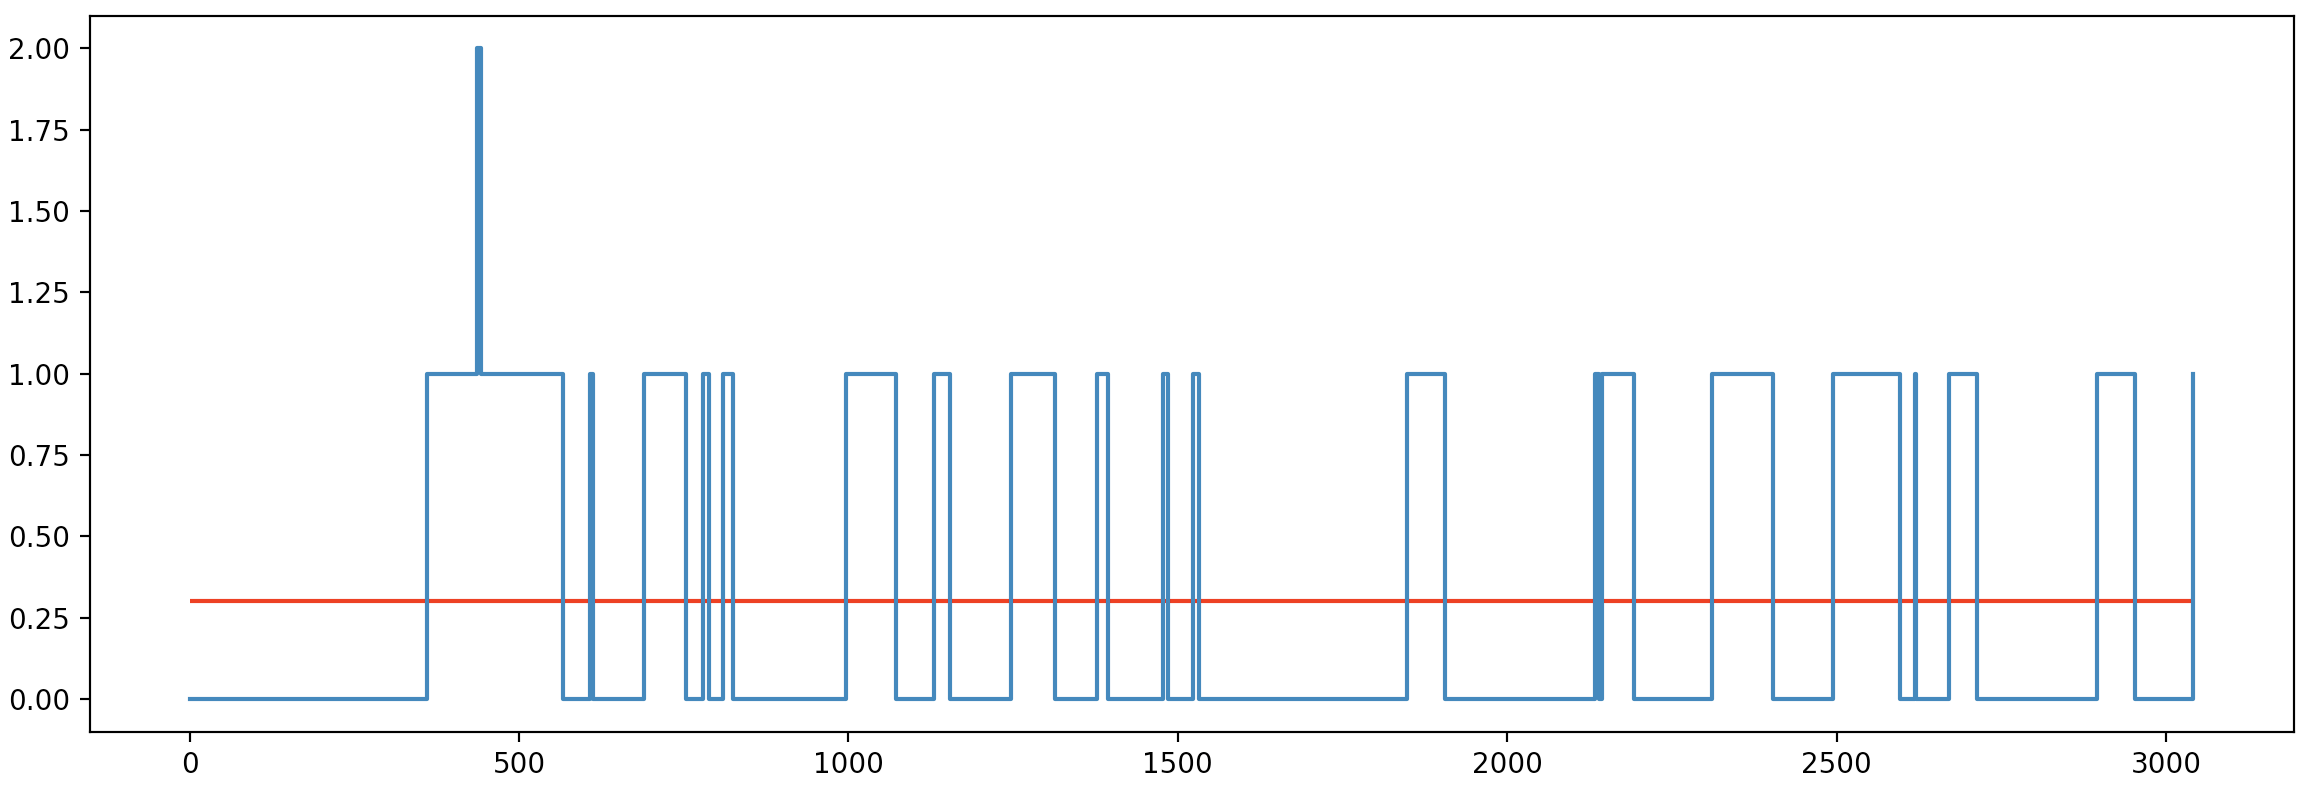
\includegraphics[width=4in]{W2_C1B.png}
\caption{The number of components in Component 1 buffer of Workstation 2}
\label{W2_C1B}
\end{center}
\end{figure}

Component 1 buffer of Workstation 2:

Verification: $L = 0.301, \lambda = 0.014, w = 21.773, T = 2713.501$
\begin{equation}
\lambda w = 0.02*28.034 = 0.301 = L
\end{equation}

This queue pass the Little's law verification.

\begin{figure}[htbp]
\begin{center}
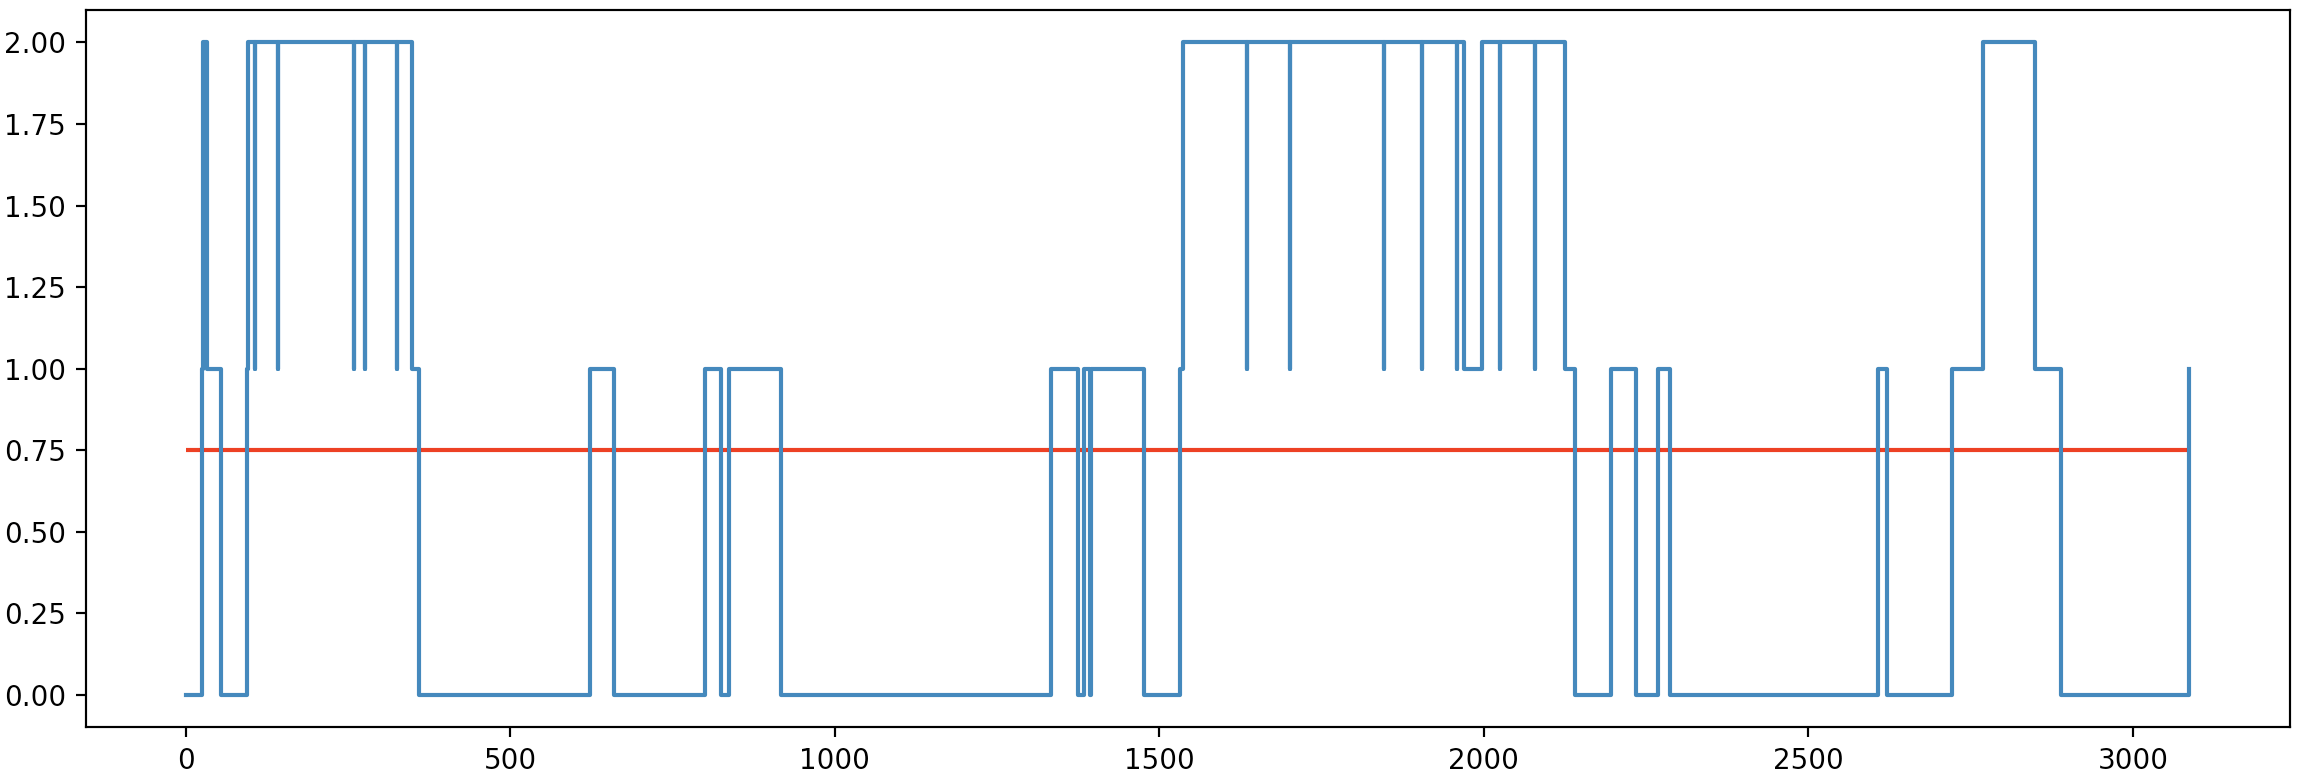
\includegraphics[width=4in]{W2_C2B.png}
\caption{The number of components in Component 2 buffer of Workstation 2}
\label{W2_C2B}
\end{center}
\end{figure}

Component 2 buffer of Workstation 2:

Verification: $L = 0.751, \lambda = 0.020, w = 37.372, T = 2713.501$
\begin{equation}
\lambda w = 0.020*37.372 = 0.751 = L
\end{equation}

This queue pass the Little's law verification.

\begin{figure}[htbp]
\begin{center}
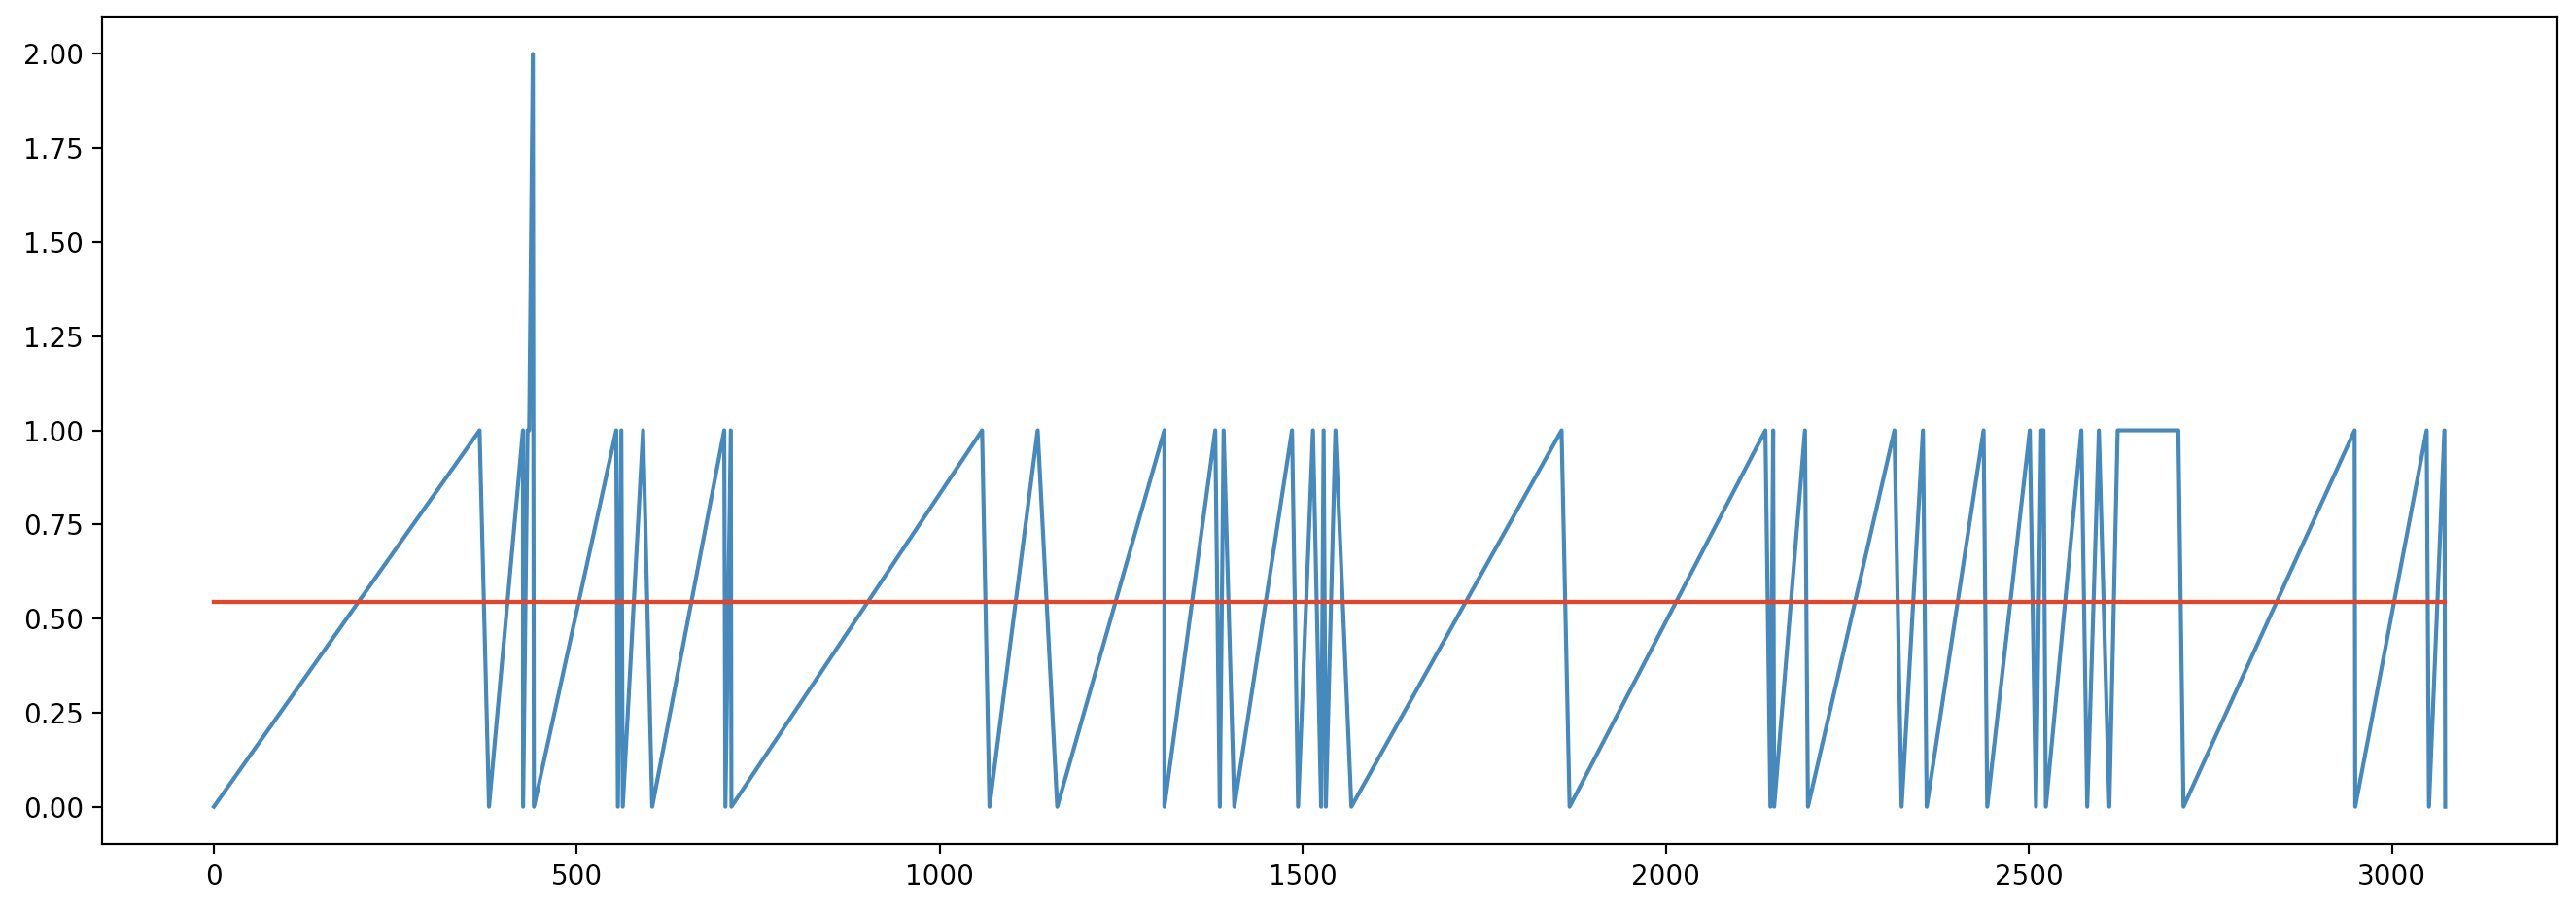
\includegraphics[width=4in]{W3_C1B.png}
\caption{The number of components in Component 1 buffer of Workstation 3}
\label{W3_C1B}
\end{center}
\end{figure}

Component 1 buffer of Workstation 3:

Verification: $L = 0.015, \lambda = 0.004, w = 3.676, T = 2713.501$
\begin{equation}
\lambda w = 0.004*3.676 = 0.015 = L
\end{equation}

This queue pass the Little's law verification.

\begin{figure}[htbp]
\begin{center}
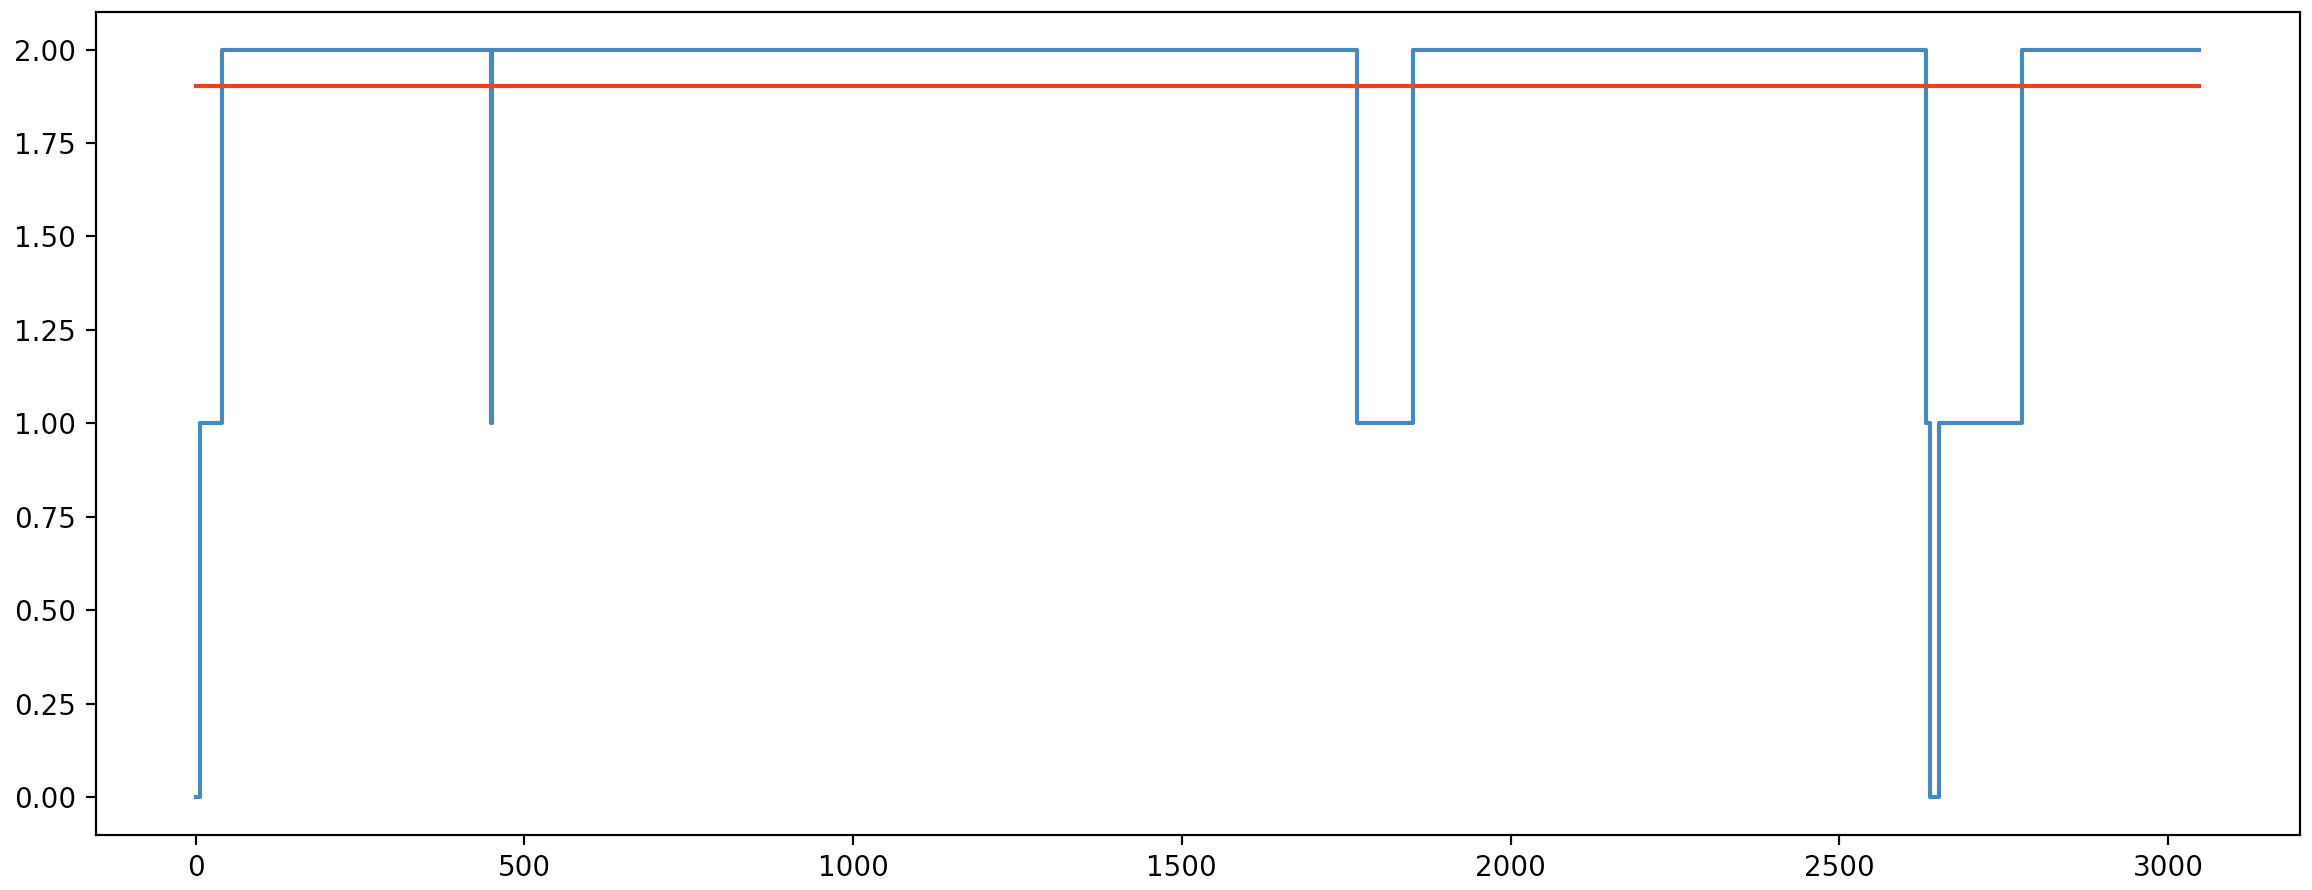
\includegraphics[width=4in]{W3_C3B.png}
\caption{The number of components in Component 3 buffer of Workstation 3}
\label{W3_C3B}
\end{center}
\end{figure}

Component 3 buffer of Workstation 3:

Verification: $L = 1.556, \lambda = 0.024, w = 64.972, T = 2713.501$
\begin{equation}
\lambda w = 0.024*64.972 = 1.556 = L
\end{equation}

This queue pass the Little's law verification.

So, all queues of this model pass the Little's law verification.

\subsection{Validation}

Validation Process

Step 1: Build a model that has high face validity

Step 2: Validate model assumptions

Step 3: Validate input-output transformations

\subsubsection{Face Validity}

The model appears reasonable. Potential users and knowledgeable people can also evaluate model output for reasonableness and can aid in identifying model deficiencies. The model is able to reflect the reality queuing systems that have events like arrival, output and block. Inspectors distribute components to correct workstations while each station prepares a buffer for each component they receive. Each buffer can temporarily store 2 components at most and it would close itself after that. The workstation gets all components it needs to produce, it takes out one component from its buffer and starts working. This model can deal with what the real scenario describes and it appears reasonable, which means I reckon it passes the face validity. 


\subsubsection{Model Assumptions}

The model assumption consists of two parts: structure assumption and data assumption. About the data assumption, we have mentioned that in the last deliverable that the data we simulate comes from the data points generator, which is validated as that can produce similar data points to reality recorded samples. Now that the generator passes Chi-square validation, we can use it to generate experimental data for us and these points are representative. For the structure part, I used Python language to build a system as what the question depicts. Each inspector and workstation is an object and python is an object-orientated program language so it's easy to achieve these functions.

\subsubsection{Input-Output Transformation}

\section{Production Runs and Analysis}
\subsection{The Length of Time in Simulation}
The length of time we record in the simulation is worth to talk. Although in workstation 1 the workstation many continuously working because it just need one component, the other two stations may stop working until the simulation ends. That is because the other two workstations needs two different kinds of gears and C2 and C3 are both provided by inspector 2 and also need C1 to start working. Of course, we can imagine in this experiment the number of C1 is not enough for both three workstations to finish their products, which means the last two components stay in the buffer for much long time until the simulation ends. So we have to arrange a good time length for them, which is a time point that no components in all workstations' buffers. That would be helpful for us to calculate the output data points. The time point is $T = 2713.501$
\subsection{Measures of Performance}
Obviously, it's a discrete time data model, which we assign $[Y_1, Y_2, ..., Y_n]$ to output. The point estimation for discrete time data is:

\begin{equation}
\hat \theta = \frac{1}{n} \sum_{i=1}^{n}Y_i
\end{equation}

We hope that $E(\hat \theta)=\theta$
The output of the system is gettable and we have confidence to evaluate it.

To make sure that what I got is in static state, I used moving average and batch average to make sure this state is representative. I made experiment 10 times longer than the transit state to make sure the state is the static state. 

Based on output distributions, suppose an output Y follows the normal distribution with mean $\theta$,
variance $\delta ^2$ (both unknown). Let $Y_i$ be the average within the $i^{th}$ replication of the simulation (its
mathematical expectation is $\theta$). Sample variance across R replications:

\begin{equation}
S^2 = {\frac{1}{R-1} \sum^{R}_{i=1} (Y_i-\bar Y)}
\end{equation}

In this experiment, I did 10 times replications to estimate the confidence interval of the outputs. As the formulation, the confidence interval would be the normally distributed.

\begin{equation}
\bar Y\pm t_{\alpha / 2, R-1}\frac{S}{\sqrt R}
\end{equation}


\subsection{Required Number of Replications}
We need to perform several independent replications of the simulation in order to obtain usable results.

In the project requirements, we stated that there must be a 0.95 confidence interval, and its width should not exceed 0.2 of the estimated value. This will perform 10 copies and then calculate each confidence interval based on the data from each copy.

\begin{table}[htp]
\caption{Replications of simulations}
\begin{center}
\begin{tabular}{cccccc}
\hline
Replications & 1 & 2 & 3 & 4 & 5\\
Inspector 1 mean time&10.288&9.928&10.580&10.293&10.753\\
Inspector 2 mean time&19.045&16.605&20.924&18.834&16.918\\
No. in Buffer W1C1&0.111&0.098&0.097&0.077&0.086\\
No. in Buffer W2C1&0.305&0.343&0.449&0.369&0.327\\
No. in Buffer W2C2&0.789&0.863&0.64&0.83&0.533\\
No. in Buffer W3C1&0.012&0.058&0.081&0.0&0.013\\
No. in Buffer W3C3&1.539&1.615&1.458&1.865&1.76\\
Wait time W1C1&1.604&1.324&1.37&1.034&1.246\\
Wait time W2C1&19.4&22.583&30.166&27.079&21.297\\
Wait time W2C2&49.251&56.495&42.706&51.525&34.173\\
Wait time W3C1&4.979&4.738&8.208&5.345&1.251\\
Wait time W3C3&122.52&133.86&149.748&192.265&180.912\\
No. P1&217.0&221.0&227.0&228.0&224.0\\
No. P2&46&44&41&41&43\\
No. P3&37&35&32&31&33\\
Idle \% Inspector 1&0.003&0.001&0.001&0.0&0.0\\
Idle \% Inspector 2&0.467&0.549&0.492&0.564&0.581\\
Idle \% Workstation 1&0.646&0.662&0.672&0.676&0.682\\
Idle \% Workstation 2&0.833&0.84&0.852&0.819&0.793\\
Idle \% Workstation 3&0.896&0.881&0.911&0.914&0.906\\
\hline


\end{tabular}



\begin{tabular}{cccccc}
\hline
Replications & 6 & 7 & 8 & 9 & 10\\
Inspector 1 mean time&10.709&8.928&9.56&9.173&10.415\\
Inspector 2 mean time&21.912&23.627&21.262&22.081&25.313\\
No. in Buffer W1C1&0.068&0.079&0.075&0.154&0.081\\
No. in Buffer W2C1&0.231&0.355&0.349&0.411&0.421\\
No. in Buffer W2C2&0.804&0.837&0.67&0.597&0.448\\
No. in Buffer W3C1&0.07&0.11&0.066&0.235&0.086\\
No. in Buffer W3C3&1.595&1.293&1.539&1.263&1.399\\
Wait time W1C1&0.933&0.934&0.947&1.895&1.147\\
Wait time W2C1&17.462&20.792&22.195&22.904&29.211\\
Wait time W2C2&59.944&44.426&37.423&34.907&24.163\\
Wait time W3C1&5.146&6.324&2.867&6.474&7.973\\
Wait time W3C3&187.601&102.066&148.534&158.581&112.173\\
No. P1&235.0&226.0&223.0&228.0&223.0\\
No. P2&39.0&42.0&43.0&41.0&44.0\\
No. P3&26.0&32.0&34.0&30.0&33.0\\
Idle \% Inspector 1&0.001&0.0&0.006&0.0&0.011\\
Idle \% Inspector 2&0.541&0.312&0.45&0.382&0.372\\
Idle \% Workstation 1&0.703&0.681&0.669&0.659&0.688\\
Idle \% Workstation 2&0.831&0.838&0.838&0.821&0.855\\
Idle \% Workstation 3&0.943&0.822&0.937&0.945&0.948\\
\hline

\end{tabular}
\end{center}
\label{default}
\end{table}%

\begin{table}[htp]
\caption{Replications of simulations}
\begin{center}
\begin{tabular}{cccc}
\hline
Statistic & Mean & Variance & Confidence Interval\\
Inspector 1 mean time&10.063&0.374&[9.625, 10.5]\\
Inspector 2 mean time&20.652&7.086&[18.748, 22.556]\\
No. in Buffer W1C1&0.093&0.001&[0.076, 0.11]\\
No. in Buffer W2C1&0.356&0.004&[0.313, 0.399]\\
No. in Buffer W2C2&0.701&0.019&[0.603, 0.799]\\
No. in Buffer W3C1&0.073&0.004&[0.027, 0.119]\\
No. in Buffer W3C3&1.533&0.033&[1.403, 1.662]\\
Wait time W1C&1.243&0.091&[1.028, 1.459]\\
Wait time W2C1&23.309&15.785&[20.467, 26.151]\\
Wait time W2C2&43.501&110.992&[35.965, 51.038]\\
Wait time W3C1&5.331&4.078&[3.886, 6.775]\\
Wait time W3C3&148.826&896.198&[127.411, 170.241]\\
No. P1&225.2&21.16&[221.909, 228.491]\\
No. P2&42.4&3.64&[41.035, 43.765]\\
No. P3&32.3&8.01&[30.275, 34.325]\\
Idle \% Inspector 1&0.002&0&[0, 0.005]\\
Idle \% Inspector 2&0.471&0.008&[0.409, 0.533]\\
Idle \% Workstation 1&0.674&0&[0.663, 0.685]\\
Idle \% Workstation 2&0.832&0&[0.82, 0.844]\\
Idle \% Workstation 3&0.91&0.001&[0.884, 0.936]\\
\hline

\end{tabular}
\end{center}
\label{default}
\end{table}%





















\end{document}